\begin{problem}{/images/problems/59_pic.jpg}{Shadow of a Rotated Cube}  We have a cube whose side lengths are equal to 1cm. We  rotate it via a random vector in 3d space. What is the expected value of the area of the shadow of the rotated cube?
\end{problem}
\begin{solution}
The answer is equal to $3/2cm^2$.\\[0.2cm]
We first point out that any vertical line whose projection on the ground lies within the shadow of the cube crosses the cube at exactly two locations (except for the edge cases that do not matter in our argument). This implies that the total area of the shadow of the cube is equal to one half of the sum of the areas of the shadows of its sides. Since the cube has 6 sides with equal areas, the average area of the shadow of the cube is equal to three times the average area of a side of the cube.

\begin{center}
	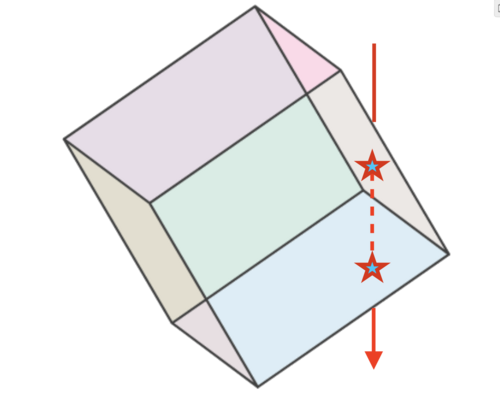
\includegraphics[width=9cm]{/images/problems/59_sol1.png}
\end{center}

Now, consider a side of the cube which is a 1cm by 1cm square as shown below.
\begin{center}
	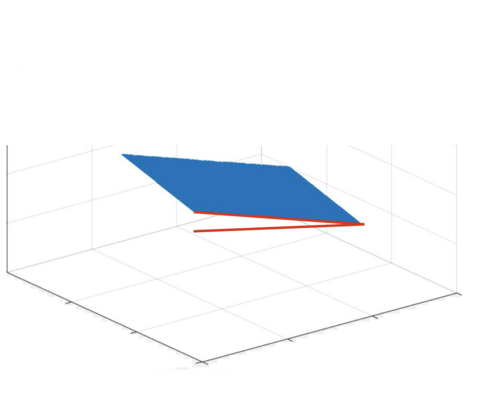
\includegraphics[width=9cm]{/images/problems/59_sol2.png}
\end{center}
It follows from basic mathematics that the area of the shadow for a rotated square is equal to the area of the square multiplied by (the absolute value of) the cosine of the angle between the rotation vector and plane $y=0$. 
Even though the rotation vector is random and the angle between the vector and plane $y=0$ is in range $(0, \pi)$, this angle is not uniformly drawn from $(0, \pi)$. More precisely, the probability that the angle of a random vector with plane $y=0$ is equal to $\theta$ is proportional to $sin(\theta)$.

 Thus, the average value of the area of the shadow of the square is equal to $1cm^2 \cdot \frac{\int_{0}^{\pi} 2\pi sin(\theta) |cos(\theta)| d_\theta}{4\pi} = 1cm^2 \cdot \int_{0}^{\pi/2}sin(\theta) cos(x) d_\theta =1/2$. This mean that the  expected value of the area of the shadow of the cube is equal to $3/2 cm^2$.
\end{solution}

